\documentclass[10pt, compress]{beamer}

\usetheme{m}

\usepackage{booktabs}
\usepackage[scale=2]{ccicons}
\usepackage{minted}
\usepackage{tikz}
\usetikzlibrary{arrows,automata,shapes,positioning,calc}


\usepgfplotslibrary{dateplot}

\usemintedstyle{trac}

\title{Projet Pensées Profondes}
\subtitle{}
\date{December 18, 2014}
\institute{École Normale Supérieure de Lyon}

\begin{document}

\maketitle

\begin{frame}[fragile]
Raphaël \textsc{Charrondière}

Marc \textsc{Chevalier}

Quentin \textsc{Cormier}

Tom \textsc{Cornebize}

Yassine \textsc{Hamoudi}

Valentin \textsc{Lorentz}

Thomas \textsc{Pellissier} \textsc{Tanon}
\end{frame}

\begin{frame}[fragile]
    \frametitle{A need of answers}
    Who was the wife of Louis Pasteur?
    \begin{figure}
        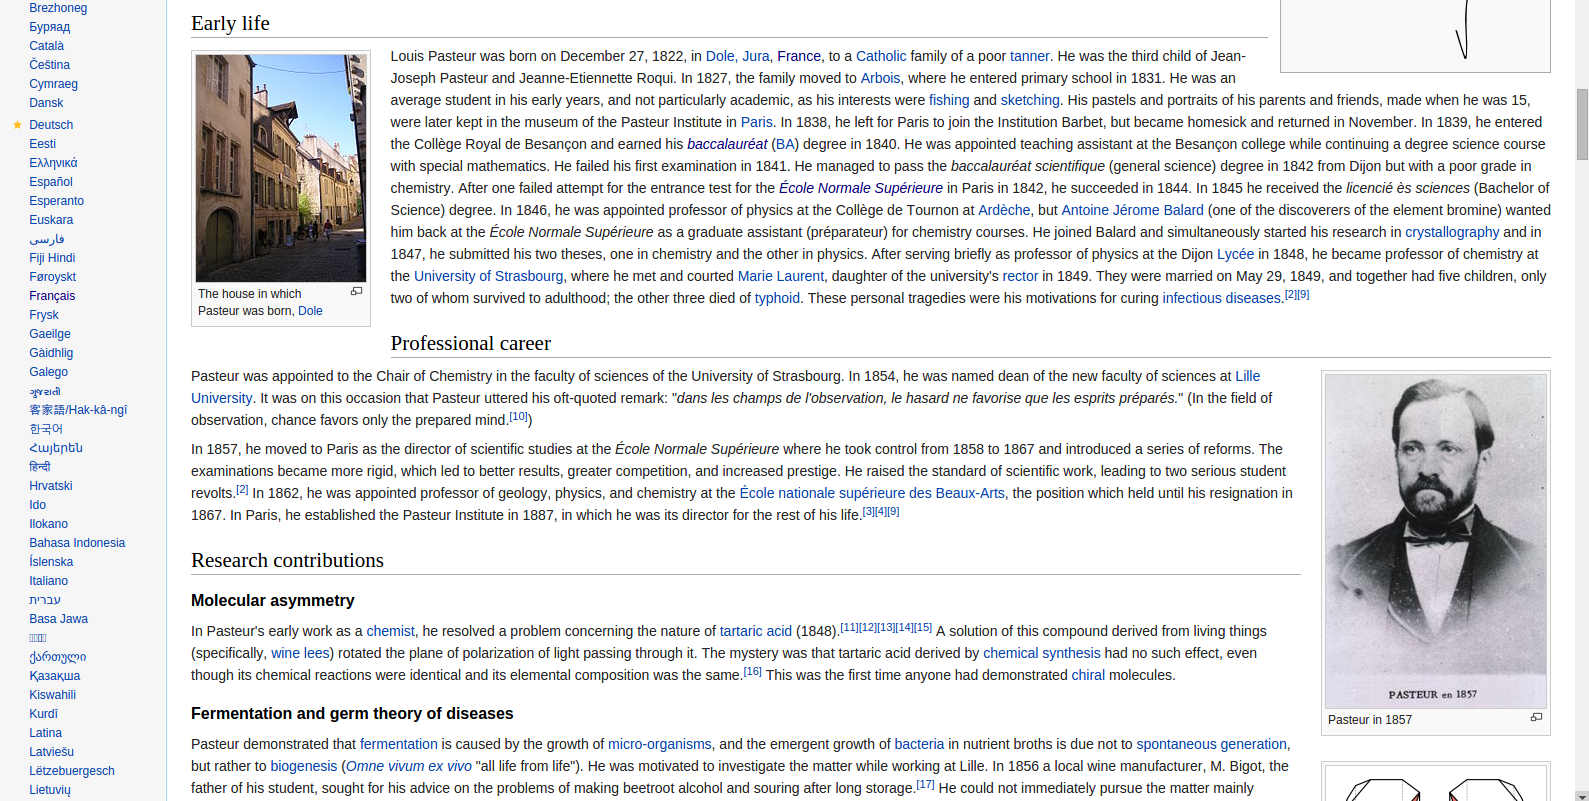
\includegraphics[width=\textwidth]{pasteurWiki.png}
    \end{figure}
\end{frame}

\begin{frame}[fragile]
    \frametitle{Existing tools}
    \begin{tabular}{ll}
        WolframAlpha & Marie Pasteur\\
        Google & Wikipeda page of Marie Pasteur\\
        Bing & Wikipeda page of Louis Pasteur\\
        Yahoo & answers.com page with this question
    \end{tabular}
\medbreak
\alert{Closed-source, bad on some questions.}
\end{frame}

\begin{frame}[fragile]
    \frametitle{PPP introduces Platypus}
    \begin{center}
        \url{http://ppp.pony.ovh/}
    \end{center}
\end{frame}

\section{Overview}

\begin{frame}[fragile]
    \frametitle{Datamodel}
\end{frame}

\begin{frame}[fragile]
    \frametitle{Architecture}
    \begin{figure}
        \resizebox{.9\linewidth}{!}{
            \newlength{\moduledistance}
\setlength{\moduledistance}{1cm}
\overfullrule=2cm
\tikzset{
    module/.style={
           rectangle,
%           rounded corners,
           draw=mDarkTeal, very thick,
           minimum width=3cm,
           minimum height = 0.7cm,
           node distance = 1.5cm,
           inner sep=2pt,
           text centered,
           },
}

\tikzset{
    core/.style={
           circle,
           draw=mDarkTeal, very thick,
           minimum width=2cm,
           inner sep=2pt,
           text centered,
           },
}

\tikzset{
    arrow/.style={
           ->,
           draw=mDarkTeal, very thick,
    }
}

\tikzset{
    darrow/.style={
           <->,
           draw=mDarkTeal, very thick,
    }
}

\begin{tikzpicture}[->,>=stealth']
    \node[core] (core) {
        Core
    };
    \node[module,
          right of=core,
          right=\moduledistance,
          ] (grammatical) {
          Grammatical
    };
    \node[module,
          below of=grammatical,
          ] (standalone) {
        \begin{tabular}{c}
        Machine Learning\\Standalone
        \end{tabular}
    };
    \node[module,
          above of=grammatical,
          ] (reformulation) {
        \begin{tabular}{c}
        Machine Learning\\Reformulation
        \end{tabular}
    };
    \node[module,
          left of=core,
          left=\moduledistance,
          ] (wikidata) {
        Wikidata
    };
    \node[module,
          above of=wikidata,
          ] (cas) {
        Computer Algebra
    };
    \node[module,
          below of=wikidata,
          ] (spellchecker) {
        Spell-checker
    };
    \node[module,
          above of=core,
          above=1cm,
          ] (webui) {
        \begin{tabular}{c}
        Web User\\
        Interface
        \end{tabular}
    };
    \node[module,
          above of=reformulation,
%          right=\moduledistance,
          ] (logging) {
        Logging backend
    };
    \draw[mLightBrown,thick] ($(reformulation.north west)+(-0.3,0.3)$)  rectangle node[yshift=-2.5cm,below] {Question Parsing} ($(standalone.south east)+(0.3,-0.3)$);
    \draw[mLightBrown,thick] ($(cas.north west)+(-0.3,0.3)$)  rectangle node[yshift=-2.5cm,below] {Other modules} ($(spellchecker.south east)+(0.3,-0.3)$);

    \draw [darrow] (core)          -- node{} (cas.south east);
    \draw [darrow] (core)          -- node{} (wikidata.east);
    \draw [darrow] (core)          -- node{} (spellchecker.north east);
    \draw [darrow] (core)          -- node{} (reformulation.south west);
    \draw [darrow] (core)          -- node{} (grammatical.west);
    \draw [darrow] (core)          -- node{} (standalone.north west);
    \draw [darrow] (core)          -- node{} (webui.south);
    \draw [darrow] (webui)         -- node{} (logging.west);
    \draw [arrow]  (logging)       -- node{} (reformulation.north);
    \draw [arrow]  (grammatical)   -- node{} (reformulation.south);

\end{tikzpicture}

        }
    \end{figure}
\end{frame}

\begin{frame}[fragile]
    \frametitle{Modules creation}
    PPP objects and communication primitives implemented in Python and PHP.

    Python module creation script.

    $\rightarrow$ Focus on your code, not the administrative details.
\end{frame}

\section{Question parsing}

\subsection{Grammatical approach}

\subsection{Machine Learning \--- Reformulation}

\subsection{Machine Learning \--- Standalone}

\section{Back-end}

\subsection{Wikidata}

\subsection{Add-ons}

\begin{frame}[fragile]
    \frametitle{Computer Algebra System}
\end{frame}

\begin{frame}[fragile]
    \frametitle{Spell Checker}
    Based on \alert{GNU Aspell}.

    \medbreak

    What are the langajes of Soth Afryka?

    $\rightarrow$

    What are the languages of South Africa?
\end{frame}

\section{Better than Wolfram?}

\begin{frame}[fragile]
    \frametitle{Nested question}

Who is the wife of the president of the United States?
    \begin{tabular}{ll}
        \alert{WolframAlpha} & Barack Obama\\
        \alert{Platypus} & Michelle Obama\\
    \end{tabular}

    \medbreak

    What are the birth dates of the daughters of the wife of the president of the United States?
    \begin{tabular}{ll}
        \alert{WolframAlpha} & Barack Obama\\
        \alert{Platypus} & Saturday, July 4, 1998 \& Sunday, June 10, 2001\\
    \end{tabular}
\end{frame}

\begin{frame}[fragile]
    \frametitle{Conjunction}

Who is an actor in Titanic and Inception?
    \begin{tabular}{ll}
        \alert{WolframAlpha} & all the actors of the two movies\\
        \alert{Platypus} & Leonardo DiCaprio\\
    \end{tabular}
\end{frame}

\section{Future work}

\begin{frame}[fragile]
    \frametitle{Better database}

    ``How fast is the TGV?''

    ``How width is a tennis court?''

    Not answered by \alert{Wikidata}.

    \medbreak

    $\rightarrow$ Improve Wikidata?

    $\rightarrow$ Use another database?
\end{frame}

\begin{frame}[fragile]
    \frametitle{Better question parsing}

    ``What is the date of birth of Isaac Newton?''

    ``In which band does Bono sing?''

    Not parsed correctly.

    \medbreak

    $\rightarrow$ Train the Stanford CoreNLP library?

    $\rightarrow$ Improve the algorithm of the Grammatical module?

    $\rightarrow$ Better datasets for the ML modules?
\end{frame}

\begin{frame}[fragile]
    \frametitle{New modules}
    \begin{table}
    \Large
    \centering
    \begin{tabular}{ccc}
        \textcolor{mLightBrown}{cooking recipes} & \textcolor{mDarkBrown}{HAL} & \textcolor{mMediumBrown}{meteo} \\
        \multicolumn{3}{c}{\textcolor{mDarkTeal}{programming language interpreter}} \\
        \textcolor{mMediumBrown}{cinema} & \textcolor{mDarkTeal}{music} & \textcolor{mLightBrown}{literature}\\
        \textcolor{mDarkBrown}{OEIS} & \textcolor{mLightBrown}{translation} & \textcolor{mDarkTeal}{chemistry}\\
        \multicolumn{3}{c}{\textcolor{mMediumBrown}{sport statistics and predictions}} \\
    \end{tabular}
    \end{table}
\end{frame}

\newlength{\logosize}
\setlength{\logosize}{12pt}
\begin{frame}[fragile]
    \frametitle{Stay tuned}
    \alert{\url{http://projetpp.github.io/}}

    \begin{tabular}{ll}
        
\includegraphics[width=\logosize]{Twitter_logo_blue.png} & \href{https://twitter.com/ProjetPP}{https://twitter.com/ProjetPP}\\
        
\includegraphics[width=\logosize]{GitHub-Mark-32px.png} &  \href{https://github.com/ProjetPP}{https://github.com/ProjetPP}\\
        
\includegraphics[width=\logosize]{ic_email_black_18dp.png} & \href{mailto:ppp@pony.ovh}{ppp@pony.ovh}\\
    \end{tabular}
\end{frame}

\plain{Questions?}

\end{document}
